\documentclass[final,3p,times,pdflatex]{elsarticle}
\usepackage[utf8x]{inputenc}      % input font encoding
\usepackage{amsmath,amssymb}
\usepackage[T1]{fontenc}          % output font encoding
\usepackage{booktabs,tabularx}
\usepackage{rotating}             % for sidewaystable
\usepackage{xspace}
\usepackage[usenames]{xcolor}
\usepackage{tikz,tikz-uml}
\usepackage{listings}
\bibstyle{elsarticle-num}
% source code highlighting
\lstset{breaklines=true,
  breakatwhitespace=true,
  stepnumber=1,
  basicstyle=\ttfamily\footnotesize,
  commentstyle=\ttfamily\color{gray},
  prebreak={\textbackslash},
  breakindent=10pt,
  breakautoindent=false,
  showspaces=false,
  showstringspaces=false,
  frame=single}
\usepackage[pdftitle={FlexibleSUSY --- A spectrum generator generator for supersymmetric models},
pdfauthor={Peter Athron,Jae-hyeon Park,Dominik Stockinger,Alexander Voigt},
pdfkeywords={FlexibleSUSY,supersymmetry,spectrum,generator,MSSM,NMSSM,E6SSM},
bookmarks=true, linktocpage]{hyperref}

%macros
\newcommand{\sarah}{SARAH\xspace}
\newcommand{\fs}{FlexibleSUSY\xspace}
\newcommand{\ESSM}{E$_6$SSM\xspace}
\newcommand{\code}[1]{\lstinline|#1|}  % inline source code
\newcommand{\textoverline}[1]{$\overline{\mbox{#1}}$}
\newcommand{\DRbar}{\textoverline{DR}}  % inline source code
\newcommand{\unit}[1]{\,\text{#1}}      % units
\DeclareMathOperator{\sign}{sign}
\def\at{\alpha_t}
\def\ab{\alpha_b}
\def\as{\alpha_s}
\def\atau{\alpha_{\tau}}
\def\oat{O(\at)}
\def\oab{O(\ab)}
\def\oatau{O(\atau)}
\def\oatab{O(\at\ab)}
\def\oatas{O(\at\as)}
\def\oabas{O(\ab\as)}
\def\oatababq{O(\at\ab + \ab^2)}
\def\oatqatababq{O(\at^2 + \at\ab + \ab^2)}
\def\oatasatq{O(\at\as + \at^2)}
\def\oatasabas{O(\at\as +\ab\as)}
\def\oatasabasatq{O(\at\as + \at^2 +\ab\as)}
\def\oatq{O(\at^2)}
\def\oabq{O(\ab^2)}
\def\oatauq{O(\atau^2)}
\def\oabatau{O(\ab \atau)}
\def\oas{O(\as)}
\def\oatauqatab{O(\atau^2 +\ab \atau )}

\journal{Computer Physics Communications}
\begin{document}
\begin{frontmatter}

 \title{\Large\bf FlexibleSUSY --- A spectrum generator generator for supersymmetric models}

\author{Peter Athron}
\address{ARC Centre of Excellence for Particle Physics at 
the Tera-scale, School of Chemistry and Physics, University of Adelaide, 
Adelaide SA 5005 Australia}
\author{Jae-hyeon Park}
\author{Dominik St\"ockinger}
\author{Alexander Voigt}
\address{Institut f\"ur Kern- und Teilchenphysik,
TU Dresden, Zellescher Weg 19, 01069 Dresden, Germany}
   
  \begin{abstract}
   Here we introduce \fs, a MATHEMATICA package which generates a C++
   spectrum generator for any SUSY model, created with modularity and
   speed in mind.  \fs makes use of the existing \sarah package
   to obtain self energies, tadpoles corrections and renormalisation
   group equations in any model.  \fs then generates C++ code for
   calculating spectra with a structure that is designed to be
   flexible. The user specifies the model supplying the
   superpotential, gauge structure and particle content in a \sarah
   model file. The user should also specify the boundary conditions in
   a separate \fs model file. {\color{red}( Do we want to keep this
     separate and in different places, add a script to put a \sarah
     model file in the right place or combine them?)}  Flexible SUSY
   then translates these into C++ code along with numerical routines
   for solving the renormalisation group equations, one loop
   electroweak symmetry breaking conditions and a solver routine for
   simultaneously solving for the spectrum.  The modular structure of
   the generated code allows for any individual component to be
   replaced with an alternative if available.  Indeed \fs has been
   intentionally designed to grow as alternative solvers and
   calculators are added.
  \end{abstract}
\begin{keyword}
sparticle, 
supersymmetry, 
Higgs
\PACS 12.60.Jv
\PACS 14.80.Ly
\end{keyword}
\end{frontmatter}

\section{Program Summary}
\noindent{\em Program title:} \fs\\ {\em Program obtainable from:}
         {\tt http://flexiblesusy.hepforge.org/}\\ {\em Distribution
           format:}\/ tar.gz\\ {\em Programming language:} {\tt
           C++}\\ {\em Computer:}\/ Personal computer\\ {\em Operating
           system:}\/ Tested on Linux 3.x\\ {\em Word size:}\/ 64
         bits\\ {\em External routines:}\/ SARAH 4.0.4, Boost library,
         lapack {\color{red} Not sure what counts here?}\\ {\em
           Typical running time:}\/ 0.1-0.3 seconds per parameter
         point.\\ {\em Nature of problem:}\/ Determining the mass
         spectrum and mixings for any supersymmetric model. The
         generated code must find simultaneous solutions to
         constraints which are specified at two or more different
         renormalisation scales, which are connected by
         renormalisation group equations forming a large set of
         coupled differential equations. \\ {\em Solution method:}\/
         Nested iterative algorithm and numerical minimisation of the
         Higgs potential.  \\ {\em Restrictions:} The couplings must
         remain perturbative at all scales between the highest and
         lowest boundary condition.  \fs~ assumes that all couplings
         of the model are real (i.e.\ $CP-$conserving)?  Due to the
         modular nature of the generated code adaption and extension
         to overcome restrictions in scope is quite straight forward.


\newpage
\section{Introduction}
Supersymmetry provides the only way to extend the space-time
symmetries of the poincar\'e group\cite{}, leading many to suspect
that it may be realised in nature in some form. In particular
supersymmetric extensions of the standard model where supersymmetry is
broken at the TeV scale have been proposed to solve the hierarchy
problem\cite{}, allow gauge coupling unification\cite{} and predict a
dark matter candidate\cite{} and can fit the observed relic
density\cite{}.  Such models have also been used for
baryogenesis\cite{} or leptogensis\cite{} to solve the
matter-anti-matter asymmetry of the universe and have been considered
as the low energy effective models originating from string
theory\cite{}.

Detailed phenonenological studies have been carried out for scenarios
with the minimal supersymmetric standard model (MSSM). Many
computational tools have been created to aid these studies and to
explore the model. In particular there are a number of public spectrum
generators for MSSM\cite{Allanach:2001kg,Porod:2003um,Djouadi:2002ze,Baer:1993ae} and two for the NMSSM\cite{Ellwanger:2006rn,Allanach:nmssm} which allow
one to find the sparticle spectrum and mixings for a particular
choices of breaking mechanism inspired boundary conditions and
specified parameters.

However none of the fundamental motivations of supersymmetry require
minimality. Yet without minimality as a constraint, constructing
specialised tools to study all relevant models would require an
enormous amount of work.  So general tools which can automate this
process and produce fats and reliable programs can greatly enhance our
ability to understand and test non-minimal realisations of
supersymmetry.

From the recent $7$ TeV and $8$ TeV runs at the Large Hadron Collider
(LHC) there have been two important developments.  First low energy
signatures expected from such models, such as the classic jets plus
missing transverse energy signature, have not been observed,
substantially raising the lower limit on sparticle masses\cite{}. No
other signature of beyond the standard model(BSM) physics has been
observed, leaving the fundamental questions which motivated BSM
physics unanswered.

 Secondly ATLAS and CMS discovered\cite{} a light Higgs of $125$ GeV,
 within the mass range that could be accommodated in the MSSM but
 requiring stops which are significantly heavier than both the direct
 collider limits and indirect limits that appears in constrained
 models from the significantly higher limits on first and second
 generation squarks.  Alternatively it is possible that a $125$ GeV
 Higgs in non-minimal models may not require such heavy stops, indeed
 a number of such models have been constructed to do exactly this by
 having new tree level contributions to the Higgs mass.

These results lead to a number of different perspectives, for example
some may wish to abandon naturalness as a motivation and focus on BSM
models which can fit the observed relic density and allow unification
of gauge couplings, while others may focus on special models which
preserve naturalness.  In both cases exploration of the models can be
aided if it is possible to quickly create a spectrum generator to find
if there are phenomenologically viable scenarios in the models they
are interested and what the general features of such models are.

\subsection{The Program}
\fs is a MATHEMATICA package designed to create a fast and easily
adaptable spectrum generator in C++ for any SUSY model and some
non-supersymmetric models {\color{red} can we?}.  \fs makes use of the
existing \sarah package \cite{Staub:2010ty,Staub:2009bi,Staub:2010jh,Staub:2012pb,Staub:2013tta} to obtain one-loop self energies, one-loop
tadpoles corrections and two-loop renormalisation group
equations(RGEs) in any model.  \fs then converts these algerbraic
expressions from \sarah into C++ code using the C++11 standard. \fs
uses some parts of SOFTSUSY\cite{Allanach:2001kg}, the very fast Eigen
library \cite{eigen}, as well as the gnu scientific library and the
boost library to create numerical routines which then use these
routines to solve the RGEs and EWSB conditions which will be used in
the spectrum generator. The main solver routine of \fs then calls
these routines to find simultaneous solutions for the EWSB, low energy
data, and other, user supplied, boundary conditions (e.g. the usual
mSUGRA universality conditions) and calculates the mass spectrum.

 The modular structure of the generated code allows for any individual
 components to be replaced with an alternative if available.  Indeed
 \fs has been intentionally designed to grow as alternative solvers
 and calculators are added and a subsequent release with an
 alternative lattice solver is already planned.{\color{red} Or Indeed
   flexible SUSY is distributed with two different main solvers, the
   two-scale solver based on the approach of \cite{} and designed for
   speed and the a lattice solver designed to solve tricky cases where
   the fixed point iteration of the two-scale approach fails to
   converge.}  In addition if one already has an existing code for
 some other purpose and simply wishes to improve upon this by adding,
 e.g, new RGEs or self energies the modular fraework makes this fairly
 straightward{\color{red} Is this true?  because it should be...}


\subsection{Design goals}

FlexibleSUSY is designed with the following points in mind:

\paragraph{Speed}
Exploring the parameter space of supersymmetric models with a high
number of free parameters is quite time consuming.  Therefore
FlexibleSUSY aims to produce spectrum generators with a short run-time.

The two most time consuming parts of a spectrum generator are the
calculation of the beta functions and the pole masses for mixed
particles.

The reason is the following: The RG solving algorithms usually need
$O(10)$ iterations to calculate a particle spectrum with $0.1\%$
precision.  During each iteration the Runge--Kutta algorithm needs to
calculate all beta functions $O(50)$ times.  Most two-loop beta
functions involve $O(50)$ matrix multiplications and additions.  All
together one arrives at $O(2.5\cdot 10^4)$ matrix multiplications.  To
optimize these matrix multiplications FlexibleSUSY uses the fast
linear algebra package \href{Eigen}{http://eigen.tuxfamily.org}, which
exploits C++ expression templates to make the matrix multiplications
easy to write and optimize.

The second most time consuming part is the precise calculation of the
pole masses for mixed particles.  For each particle $\psi_i$ the full
self-energy matrix $\Sigma^\psi_{ij}(p=m^\text{tree}_{\psi_i})$ has to
be evaluated.  Each self-energy matrix entry again involves the
evaluation of $O(50)$ Feynman diagrams, which involves the calculation
of vertices and loop functions.  All in all, one arrives at $O(500)$
Feynman diagram or $O(3\cdot 10^4)$ loop function evaluations.  To
speed up the calculation of the pole masses FlexibleSUSY makes use of
multi-threading, where each pole mass is calculated in a separate
thread.  By this technique one can gain a speed-up of $20$--$30\%$.

\paragraph{Modularity}
The large variety of supersymmetric models makes it likely that the
user needs to modify the generated spectrum generator source code.
FlexibleSUSY uses object orientation with C++ to modularize the source
code to make it easy for the user to modify and extend the spectrum
generator.  An important application here are the constraints: The RG
solvers provide a constraint interface,
\figurename~\ref{fig:schematic-two-scale-constraint-interface},
%
\begin{figure}
  \centering
  \tikzumlset{fill class=white}
  \begin{tikzpicture}
    \umlclass[x=0, y=0]{RGFlow$<$Two\_scale$>$}{}{
      + solve()
    }
    \umlclass[x=6, y=0, type=abstract]{Constraint$<$Two\_scale$>$}{}{
      + \umlvirt{apply()}\\
      + \umlvirt{get\_scale() : double}
    }
    \umlclass[x=6, y=-3]{MyConstraint}{}{
      + apply()\\
      + get\_scale() : double
    }
    \umldep{RGFlow$<$Two\_scale$>$}{Constraint$<$Two\_scale$>$}
    \umlinherit{MyConstraint}{Constraint$<$Two\_scale$>$}
  \end{tikzpicture}
  \caption{Schematic two-scale constraint interface}
  \label{fig:schematic-two-scale-constraint-interface}
\end{figure}
%
which can be implemented to create the custom constraint
\code{MyConstraint}.  In the \code{apply()} function the constraint
application takes place and the \code{get_scale()} function specifies
the scale at which the constraint is to be applied.

\section{Download and compilation}
Flexible SUSY can be downloaded from \url{http://flexiblesusy.hepforge.org}.  
To use FlexibleSUSY please make sure you have the following installed.  
\begin{itemize}
\item Mathematica, version 7 or higher
\item SARAH, version 4.0.4 or higher \url{http://sarah.hepforge.org}
\item C++11 compatible compiler (g++ 4.6.0 or higher, clang++ 3.1 or
  higher)
\item Fortran compiler (gfortran, ifort etc.)
\item Eigen library, version 3.1 \url{http://eigen.tuxfamily.org}
\item Boost library, version 1.36.0 or higher
  \url{http://www.boost.org}
\item GNU scientific library \url{http://www.gnu.org/software/gsl/}
\item lapack (needed for the Lattice algorithm only)
  \url{http://www.netlib.org/lapack/}
\end{itemize}
%
Optional:
%
\begin{itemize}
\item Looptools, version 2.8 or higher
  \url{http://www.feynarts.de/looptools/}
\end{itemize}

\subsection{Quick Start}
Create a MSSM spectrum generator
  \begin{lstlisting}[language=bash]
$ ./createmodel --models=MSSM
$ ./configure --with-models=MSSM
$ make
  \end{lstlisting}
Run the spectrum generator using the default parameter point
  \begin{lstlisting}[language=bash]
$ ./models/MSSM/run_MSSM.x
  \end{lstlisting}
Run the spectrum generator using a SLHA input file
  \begin{lstlisting}[language=bash]
$ ./models/MSSM/run_MSSM.x --slha-input-file=templates/MSSM/LesHouches.in.MSSM --slha-output-file=LesHouches.out.MSSM
  \end{lstlisting}%% $

\section{Stucture of the spectrum generator}

\subsection{Model parameters and RGEs}
Even in the simplest supersymmetric model the RGEs form a very large
set of coupled non-linear differential equations.  In a general
(softly broken) supersymmetric theory the soft-breaking parameters
depend on themselves and the susy parameters.  However, the susy
parameters are independent of the soft-breaking parameters [cite: MV,
Staub, Sperling].  This makes it possible to split the model
parameters and their into the following two subsets:
%
\begin{enumerate}
\item \emph{susy parameters:} gauge couplings, superpotential
  parameters and VEVs and
\item soft-breaking parameters.
\end{enumerate}
%
The susy parameters together with their two-loop renormalisation group
equations for the are stored in the class
\code{<model>_susy_parameters}.  The soft-breaking model parameters
together with their two-loop renormalisation group equations for the
are stored in the class \code{<model>_soft_parameters}.  The
dependence of the soft-breaking parameters on the susy parameters is
implemented via inheritance, see
\figurename~\ref{fig:parameter-classes}.
%
\begin{figure}
  \centering
  \tikzumlset{fill class=white}
  \begin{tikzpicture}
    \umlclass[x=0, y=3]{model\_susy\_parameters}{
      - susy parameters
    }{
      + beta()
    }
    \umlclass[x=0, y=0]{model\_soft\_parameters}{
      - soft-breaking parameters
    }{
      + beta()
    }
    \umlinherit{model\_soft\_parameters}{model\_susy\_parameters}
  \end{tikzpicture}
  \caption{Model parameter class structure.}
  \label{fig:parameter-classes}
\end{figure}

\subsection{Boundary conditions}
In \fs the RGE boundary conditions are implemented by inheriting from
a common \code{Constraint<Two\_scale>} interface class and
implementing the pure virtual functions \code{apply()},
\code{get\_scale()} and \code{set\_model()}, see
\figurename~\ref{fig:schematic-two-scale-constraint-interface}.  Per
default, \fs creates three default boundary conditions:
%
\begin{itemize}
\item \emph{GUT constraint:} Here the \code{apply()} function
  calculates the value of the unification scale $M_X$ (from the
  condition given in \code{HighScale}) and sets the model parameters
  given in \code{HighScaleInput}.
\item \emph{SUSY constraint:} Here the \code{apply()} function
  calculates the value of the susy scale $M_S$ and sets the model
  parameters given in \code{SUSYScaleInput}.  Afterwards the EWSB
  conditions are solved for the parameters given in
  \code{EWSBOutputParameters} at the one-loop level, i.e., the the
  parameters in \code{EWSBOutputParameters} are determined such that
  the one-loop effective potential is minimized.
\item \emph{Low-scale constraint:} This constraint matches the gauge
  and Yukawa couplings of the susy model to the Standard Model values
  using threshold corrections.  Furthermore the parameters given in
  \code{LowScaleInput} are set.
\end{itemize}

{\color{red}Different types, how we match to low energy data.
  reference EWSB or merge that section here.  mention two loop qcd
  parts from softsusy.}

\subsubsection{Electroweak symmetry breaking}
In \fs the one-loop electroweak symmetry breaking conditions are
formulated as
%
\begin{align}
  0 = \frac{\partial V^\text{tree}}{\partial v_i} - t_i,
  \label{eq:one-loop-ewsb-eq}
\end{align}
%
where $V^\text{tree}$ is the tree-level Higgs potential, $v_i$ is the
VEVs corresponding to the Higgs field $H_i$ and $t_i$ is the one-loop
tadpole diagram of $H_i$.

The electroweak symmetry breaking conditions
\eqref{eq:one-loop-ewsb-eq} are then solved simultaneously using the
iterative multi-dimensional root finder algorithm
\code{gsl_multiroot_fsolver_hybrid} from the Gnu Scientific Libraray
(GSL).  If no root was found, the \code{gsl_multiroot_fsolver_hybrids}
algorithm is tried as alternative, which uses a variable step size but
might be a little slower.

For example in the MSSM \fs expresses \eqref{eq:one-loop-ewsb-eq} as
the function
%
\begin{lstlisting}[language=C++]
int MSSM<Two_scale>::tadpole_equations(const gsl_vector* x, void* params, gsl_vector* f)
{
   ...

   const CLASSNAME::Ewsb_parameters* ewsb_parameters
      = static_cast<CLASSNAME::Ewsb_parameters*>(params);
   MSSM* model = ewsb_parameters->model;
   const unsigned ewsb_loop_order = ewsb_parameters->ewsb_loop_order;

   double tadpole[number_of_ewsb_equations];

   model->set_BMu(gsl_vector_get(x, 0));
   model->set_Mu(INPUT(SignMu) * Abs(gsl_vector_get(x, 1)));

   // calculate tree-level tadpole eqs.
   tadpole[0] = model->get_ewsb_eq_vd();
   tadpole[1] = model->get_ewsb_eq_vu();

   // subtract one-loop tadpoles
   if (ewsb_loop_order > 0) {
      model->calculate_DRbar_parameters();
      tadpole[0] -= Re(model->tadpole_hh(0));
      tadpole[1] -= Re(model->tadpole_hh(1));

   }

   for (std::size_t i = 0; i < number_of_ewsb_equations; ++i)
      gsl_vector_set(f, i, tadpole[i]);

   return GSL_SUCCESS;
}
\end{lstlisting}
%
Here \code{x} is the vector of EWSB output parameters
(\code{EWSBOutputParameters}) and \code{f} is a vector which contains
the one-loop EWSB eqs.\ \eqref{eq:one-loop-ewsb-eq}.  This
\code{tadpole_equations()} function is called inside of
\code{MSSM<Two_scale>::solve_ewsb_iteratively_with} then via
%
\begin{lstlisting}[language=C++]
// initial guess
double x_init[number_of_ewsb_equations];
ewsb_initial_guess(x_init);

// setup root finder
int ewsb_loop_order = 1;
Ewsb_parameters params = {this, ewsb_loop_order};
Root_finder<number_of_ewsb_equations> root_finder(
                           MSSM<Two_scale>::tadpole_equations,
                           &params,
                           number_of_ewsb_iterations,
                           ewsb_iteration_precision);
root_finder.set_solver_type(gsl_multiroot_fsolver_hybrid);

root_finder.find_root(x_init);
\end{lstlisting}

If higher accuracy is required additional routines with higher order
corrections can be added in a very simple way.  For example in the
MSSM by default \fs adds two loop Higgs FORTRAN routines supplied by
P.~Slavich from \cite{slavich-degrassi} to add two loop corrections of
$\oatas$, $\oabas$, $\oatq$, $\oabatau$, $\oabq$, $\oatauq$ and
$\oatab$ as follows...  Something similar is done for the NMSSM, but
in this case the NMSSM $\oatas$, $\oabas$ pieces come from
\cite{Degrassi:2009yq}.  Corrections from other sources can be added
to the generated code by...

\subsection{Tree-level spectrum}
The tree-level $\overline{DR}$ masses are calculated by diagonalizing
the mass matrices returned from \code{SARAH`MassMatrix[]}.  The
numerical diagonalization is performed by the Eigen library routines
\code{Eigen::JacobiSVD} and \code{Eigen::SelfAdjointEigenSolver} for
small matrices, and the Lapack routines \code{zgesvd}, \code{dgesvd},
\code{zheev}, \code{dsyev} for matrices with more than four rows and
columns.

\subsection{Two-scale fixed point iteration}
The default two-scale RG solver uses above beta functions and boundary
conditions to find the full set of $\overline{DR}$ masses in the model
consistent with all constraints.  It does so by iterating between the
scales of all boundary conditions, applying the constraints and
checking for convergence.  This approach is decribed in
\cite{Barger:1993gh} for the MSSM and is widely implemented in SUSY
spectrum generators.

The in more detail the two-scale algorithm used in \fs works as
follows:
%
\\Initial guess:
\begin{enumerate}
\item Guess gauge couplings $g_{1,2,3}$ at $m_Z$
\item Apply user-defined low-scale constraint (\code{LowScaleInput})
\item Guess Yukawa couplings $y^{u,d,e}_{ij}$ at $m_Z$
\item Run model to the high-scale (\code{HighScaleFirstGuess})
\item Apply high-scale constraint (\code{HighScaleInput})
\item Run model to the low-scale (\code{LowScaleFirstGuess})
\item Solve EWSB eqs.\ at the tree-level
\item Calculate \DRbar\ masses
\end{enumerate}
%
Solving the renormalization group equations:
\begin{enumerate}
\item \label{rge-step-one} Run model to the low-scale (\code{LowScale})
  \begin{enumerate}
  \item Calculate \DRbar\ masses
  \item Recalculate low-scale
  \item Calculate \DRbar\ gauge and Yukawa couplings $g_{1,2,3}$, $y^{u,d,e}_{ij}$
  \item Apply user-defined low-scale constraint (\code{LowScaleInput})
  \end{enumerate}
\item Run model to the high-scale (\code{HighScale})
  \begin{enumerate}
  \item Recalculate high-scale
  \item Apply high-scale constraint (\code{HighScaleInput})
  \end{enumerate}
\item Run model to the susy-scale (\code{SUSYScale})
  \begin{enumerate}
  \item Calculate \DRbar\ masses
  \item Recalculate low-scale
  \item Apply susy-scale constraint (\code{SUSYScaleInput})
  \item Solve EWSB eqs.\ at the one-loop level
  \end{enumerate}
\item If not converged yet, goto \ref{rge-step-one}
\end{enumerate}
%
Calculating the particle spectrum:
\begin{enumerate}
\item Run model to the susy-scale
\item Calculate the pole masses
\item Run model to the parameter output scale (SLHA block MODSEL 12)
\end{enumerate}

\begin{figure}[tb]
  \centering
  \tikzumlset{fill class=white}
  \begin{tikzpicture}
    \umlclass[x=0, y=0, type=abstract]{Beta\_function}{
      -- scale : double\\
      -- loops : unsigned\\
      -- numPars : unsigned
    }{
      + \umlvirt{display() : const Eigen::ArrayXd} \\
      + \umlvirt{set(v : const Eigen::ArrayXd\&) : void}\\
      + \umlvirt{beta() : Eigen::ArrayXd}\\
      + run\_to(scale : double, eps : double) : void\\
    }
    \umlclass[x=8, y=-12, template={T}]{MSSM}{}{}
    \umlclass[x=8, y=-8, type=abstract]{Two\_scale\_model}{}{
      + \umlvirt{calculate\_spectrum() : void}\\
      + \umlvirt{run\_to(scale : double, eps : double) : void}\\
      + \umlvirt{set\_precision(precision : double) : void}
    }
    \umlclass[x=0, y=-4]{MSSM\_susy\_parameters}{}{
      + display() : const Eigen::ArrayXd \\
      + set(v : const Eigen::ArrayXd\&) : void\\
      + beta() : Eigen::ArrayXd
    }
    \umlclass[x=0, y=-8]{MSSM\_soft\_parameters}{}{
      + display() : const Eigen::ArrayXd \\
      + set(v : const Eigen::ArrayXd\&) : void\\
      + beta() : Eigen::ArrayXd
    }
    \umlclass[x=0, y=-12]{MSSM$<$Two\_scale$>$}{}{
      + calculate\_spectrum() : void\\
      + run\_to(scale : double, eps : double) : void\\
      + set\_precision(precision : double) : void
    }
   \umlinherit{MSSM\_susy\_parameters}{Beta\_function}
   \umlinherit{MSSM\_soft\_parameters}{MSSM\_susy\_parameters}
   \umlinherit{MSSM$<$Two\_scale$>$}{MSSM\_soft\_parameters}
   \umlinherit{MSSM$<$Two\_scale$>$}{Two\_scale\_model}
   \umldep[arg1={$<<$bind$>>$}, mult1={T $\rightarrow$ Two\_scale}, pos1=0.5]{MSSM$<$Two\_scale$>$}{MSSM}
  \end{tikzpicture}
  \caption{Two-scale model class hierarchy}
  \label{fig:two-scale-model-class-hierarchy}
\end{figure}

\begin{figure}[tb]
  \centering
  \tikzumlset{fill class=white}
  \begin{tikzpicture}
    \umlclass[x=0, y=0, type=abstract]{Two\_scale\_model}{}{
      + \umlvirt{calculate\_spectrum() : void}\\
      + \umlvirt{run\_to(scale : double, eps : double) : void}\\
      + \umlvirt{set\_precision(precision : double) : void}
    }
    \umlclass[x=0, y=-4]{RGFlow$<$Two\_scale$>$}{}{
      + solve() : void
    }
    \umlclass[x=8, y=0]{Constraint$<$Two\_scale$>$}{}{
      + \umlvirt{apply() : void}\\
      + \umlvirt{get\_scale() : double}\\
      + \umlvirt{set\_model(model : Two\_scale\_model*) : void}
    }
    \umlclass[x=8, y=4, template={T}]{Constraint}{}{}
    \umlclass[x=0, y=-7]{Initial\_guesser$<$Two\_scale$>$}{}{
      + \umlvirt{guess() : void}
    }
    \umlclass[x=0, y=-11, template={T}]{Initial\_guesser}{}{}
    \umlclass[x=8, y=-7]{Convergence\_tester$<$Two\_scale$>$}{}{
      + \umlvirt{accuracy\_goal\_reached() : bool}\\
      + \umlvirt{max\_iterations() : unsigned}
    }
    \umlclass[x=8, y=-11, template={T}]{Convergence\_tester}{}{}
    \umlclass[x=8, y=-4, template={T}]{RGFlow}{}{}
    \umldep[arg1={$<<$bind$>>$}, mult1={T $\rightarrow$ Two\_scale}, pos1=0.5]{RGFlow$<$Two\_scale$>$}{RGFlow}
    \umldep[mult1=1..*]{RGFlow$<$Two\_scale$>$}{Two\_scale\_model}
    \umldep[mult1=1..*]{RGFlow$<$Two\_scale$>$}{Constraint$<$Two\_scale$>$}
    \umldep{RGFlow$<$Two\_scale$>$}{Initial\_guesser$<$Two\_scale$>$}
    \umldep{RGFlow$<$Two\_scale$>$}{Convergence\_tester$<$Two\_scale$>$}
    \umldep[mult1={$<<$bind$>>$}, arg1={T $\rightarrow$ Two\_scale}, pos1=0.5]{Initial\_guesser$<$Two\_scale$>$}{Initial\_guesser}
    \umldep[mult1={$<<$bind$>>$}, arg1={T $\rightarrow$ Two\_scale}, pos1=0.5]{Convergence\_tester$<$Two\_scale$>$}{Convergence\_tester}
    \umldep[arg1={$<<$bind$>>$}, mult1={T $\rightarrow$ Two\_scale}, pos1=0.5]{Constraint$<$Two\_scale$>$}{Constraint}
  \end{tikzpicture}
  \caption{Two-scale renormalization group solver class hierarchy}
  \label{fig:two-scale-rgflow-class-hierarchy}
\end{figure}
{\color{red} copied and pasted from latest manual -- not sure how best to maintain this, could split maual up into tiny bits, but we may also want some differences?}

\subsection{Pole masses}
After the solver routine has finished and convergence has been
achieved, all $\overline{DR}$ parameters are consistent with the
one-loop EWSB conditions, low energy data and all user supplied
boundary conditions are known at any scale between \code{LowScale} and
\code{HighScale}.

The physical (pole) mass spectrum can now be calculated.  \fs uses the
full one-loop self-energies and tree-level mass matrices to calculate
the pole masses at the one-loop level.  If higher accuracy is required
additional routines with higher order corrections can be added in a
very simple way. For example in the MSSM by default \fs adds two-loop
Higgs FORTRAN routines supplied by P.~Slavich from
\cite{slavich-degrassi} to add two loop corrections of $\oatas$,
$\oabas$, $\oatq$, $\oabatau$, $\oabq$, $\oatauq$ and $\oatab$ as
follows... {\color{red} This is not yet implemented!}

Something similar is done for the NMSSM, but in this case the NMSSM
$\oatas$, $\oabas$ pieces come from \cite{Degrassi:2009yq}, while for
$\oatq$, $\oabatau$, $\oabq$, $\oatauq$ and $\oatab$ the MSSM pieces
are used though it should be understood that these are not complete in
the NMSSM. For other models since the Higgs mass is a very important
measurement and the two loop corrections can be larger than the
current experimental error \cite{Degrassi:2009yq} we recommend that
the leading log two loop corrections are estimated, by generalising
those of the MSSM or NMSSM, as has been done, for example, in the
E$_6$SSM\cite{King:2005jy}.  {\color{red} This is not yet implemented!}

Corrections to other masses or further corrections to the Higgs states
can be added very easily by...

\section{Implementing new models}
\section{Adapting the code at the C++ level}
\section{Using individual modules in your own code}

\section{Run-time comparison with other spectrum generators}

We compare the run-time of the four different spectrum generators
FlexibleSUSY (version 0.5.3), Softsusy (version 3.4.0), SPheno
(3.2.4), SPhenoMSSM (generated with SARAH 4.1.0 and linked against
SPheno 3.2.4).  FlexibleSUSY and Softsusy were compiled with g++ 4.8.0
and gfortran 4.8.0.  SPheno and SPhenoMSSM were compiled with Intel
ifort 13.1.3 20130607\footnote{We are using Intel's ifort compiler,
  instead of gfortran 4.8.0, because it decreases the run-time of
  SPheno and SPhenoMSSM by approximately a factor $1.5$.}.  We're
generating random CMSSM parameter points with $m_0\in [50,1000]$
$m_{1/2}\in [50,1000]$, $\tan\beta\in [1,100]$, $\sign\mu\in
\{-1,+1\}$ and $A_0\in [-1000,1000]$.  The following SLHA template
file was used:
%
\begin{verbatim}
Block MODSEL                 # Select model
    6    0                   # flavour violation
    1    1                   # mSUGRA
Block SMINPUTS               # Standard Model inputs
    1   1.279180000e+02      # alpha^(-1) SM MSbar(MZ)
    2   1.166390000e-05      # G_Fermi
    3   1.189000000e-01      # alpha_s(MZ) SM MSbar
    4   9.118760000e+01      # MZ(pole)
    5   4.200000000e+00      # mb(mb) SM MSbar
    6   1.709000000e+02      # mtop(pole)
    7   1.777000000e+00      # mtau(pole)
Block SOFTSUSY               # SOFTSUSY specific inputs
    1   1.000000000e-04      # tolerance
    2   2                    # up-quark mixing (=1) or down (=2)
    3   0                    # printout
    5   1                    # 2-loop running
    7   2                    # EWSB and Higgs mass loop order
Block FlexibleSUSY
    0   1.000000000e-04      # precision goal
    1   0                    # max. iterations (0 = automatic)
    2   0                    # algorithm (0 = two_scale, 1 = lattice)
    3   0                    # calculate SM pole masses
    4   1                    # calculate loop masses
    5   1                    # EWSB loop order
Block SPhenoInput            # SPheno specific input
    1  -1                    # error level
    2   1                    # SPA conventions
    11  0                    # calculate branching ratios
    13  0                    # include 3-Body decays
    12  1.000E-04            # write only branching ratios larger than this value
    31  -1                   # fixed GUT scale (-1: dynamical GUT scale)
    32  0                    # Strict unification
    34  1.000E-04            # Precision of mass calculation
    35  40                   # Maximal number of iterations
    37  1                    # Set Yukawa scheme
    38  2                    # 1- or 2-Loop RGEs
    50  1                    # Majorana phases: use only positive masses
    51  0                    # Write Output in CKM basis
    52  0                    # Write spectrum in case of tachyonic states
    55  1                    # Calculate one loop masses
    57  0                    # Calculate low energy constraints
    60  0                    # Include possible, kinetic mixing
    65  1                    # Solution tadpole equation
    75  0                    # Write WHIZARD files
    76  0                    # Write HiggsBounds file
    86  0.                   # Maximal width to be counted as invisible in Higgs decays
    510 0.                   # Write tree level values for tadpole solutions
    515 0                    # Write parameter values at GUT scale
    520 0.                   # Write effective Higgs couplings (HiggsBounds blocks)
    525 0.                   # Write loop contributions to diphoton decay of Higgs
Block MINPAR
    1   [50..1000]           # m0(MX)
    2   [50..1000]           # m12(MX)
    3   [1..100]             # tan(beta)(MZ) DRbar
    4   {-1,+1}              # sign(mu)
    5   [-1000..1000]        # A0(MX)
\end{verbatim}
%
The SLHA file was passed to each spectrum generator and the
(wall-clock) time was measured until the program has finished.  The
average run-times for three different CPU types can be found in
\tablename~\ref{tab:run-time-comparison}.  The first row shows the
run-time on a Intel Core2 Duo (P8600) where only one core was enabled.
The second row shows the run-time on a Intel Core2 Duo (P8600) where
both cores were enabled.  In the third row a Intel Xeon (L5640) was
used, which has $6$ CPU cores.
%
\begin{table}[tbh]
  \centering
  \begin{tabular}{llll}
    \toprule
                          & Intel Core2 Duo (P8600)    & Intel Core2 Duo (P8600)     & Intel Xeon (L5640)\\
                          & (1 core, $2.40\unit{GHz}$) & (2 cores, $2.40\unit{GHz}$) & (6 cores, $2.27\unit{GHz}$)\\
    \midrule
    FlexibleSUSY 0.5.3    & $0.151\unit{s}$    & $0.114\unit{s}$   & $0.081\unit{s}$\\
    Softsusy 3.4.0        & $0.178\unit{s}$    & $0.174\unit{s}$   & $0.157\unit{s}$\\
    SPheno 3.2.4          & $0.120\unit{s}$    & $0.118\unit{s}$   & $0.108\unit{s}$\\
    SPhenoMSSM 4.1.0${}^*$ & $0.463\unit{s}$    & $0.450\unit{s}$   & $0.403\unit{s}$\\
    \bottomrule
  \end{tabular}
  \caption{Average run-time for random CMSSM parameter points.
    FlexibleSUSY and Softsusy were compiled
    with g++ 4.8.0 and gfortran 4.8.0.  SPheno and SPhenoMSSM were
    compiled with ifort 13.1.3 20130607.
    ${}^*$ SPhenoMSSM was generated with SARAH 4.1.0 and linked
    against SPheno 3.2.4.}
  \label{tab:run-time-comparison}
\end{table}
%
We find that on the single-core machine SPheno is fastest with
$0.120\unit{s}$, and FlexibleSUSY is second with $0.151\unit{s}$.  In
the case of 2 or 6 CPU cores, FlexibleSUSY is fastest with
$0.114\unit{s}$ and $0.081\unit{s}$, respectively.  The reason is that
FlexibleSUSY calculates each pole mass in a separate thread, and
therefore benefits from multi-core CPUs.

\appendix
\section{Examples}
\subsection{NMSSM}
Detailed steps to create NMSSM model file.
\begin{enumerate}
\item Create new directory \code{mkdir myNMSSM}
\item Move into this new directory \code{cd myNMSSM}
\item copy the MSSM model file in \code{cp /path/to/SARAH/Models/MSSM/MSSM.m  myNMSSM.m}
\item Edit myNMSSM.m as follows
\begin{enumerate}
\item  Change Model name, author and date
\item Add singlet superfield to SuperFields
\begin{lstlisting}
SuperFields[[8]] = {s, 1, sR,    0, 1,  1, RpM};
\end{lstlisting}
\item Modify superpotential
\begin{lstlisting}
SuperPotential = Yu u.q.Hu - Yd d.q.Hd - Ye e.l.Hd + \[Lambda] s.Hu.Hd +  \[Kappa]/3 s.s.s ;
\end{lstlisting}
\item Add new VEV
\begin{lstlisting} 
  DEFINITION[EWSB][VEVs]= 
  { {SHd0, {vd, 1/Sqrt[2]}, {sigmad, \[ImaginaryI]/Sqrt[2]},{phid,1/Sqrt[2]}},
    {SHu0, {vu, 1/Sqrt[2]}, {sigmau, \[ImaginaryI]/Sqrt[2]},{phiu,1/Sqrt[2]}},
    {SsR,  {vs, 1/Sqrt[2]}, {sigmaS, \[ImaginaryI]/Sqrt[2]},{phiS,1/Sqrt[2]}}
};
\end{lstlisting}
\item  Add the singlino to the list of gauge eigenstate dirac fermions
\begin{lstlisting}
  DEFINITION[GaugeES][DiracSpinors]={
 .............
  FS -> {FsR,conj[FsR]}   
};
\end{lstlisting}
\item Edit mass eigenstates to give how the gauge eigenstates mix into mass eigenstates.  Here we add to the cp even higgs a real singlet, to the CP odd the imaginary part of the singlet and finally to the neutralinos we add the singlino.

\begin{lstlisting}
 DEFINITION[EWSB][MatterSector]= 
{   ................
    ................
     {{phid, phiu, phiS}, {hh, ZH}},      
     {{sigmad, sigmau, sigmaS}, {Ah, ZA}},
    ................
     {{fB, fW0, FHd0, FHu0, FsR}, {L0, ZN}},
     ...............
}; 

\end{lstlisting}
\end{enumerate}
\item Now we copy over particles.m \code{cp /path/to/SARAH/Models/MSSM/particles.m  ./}
\item Edit particles.m as follows
\begin{enumerate}  
\item First we add to particleDefinitions[GaugeES]:
\begin{lstlisting}
 ParticleDefinitions[GaugeES] = {
      {SsR, { Description -> "Singlet"}},        
      {FS,   { Description -> "Singlino" }},    
      ............
      };
\end{lstlisting}
Note that we are brief in information here becasue there is already some information contained in the default particles.m file in the model directory:
\begin{lstlisting} 
{{ Description -> "Singlet", 
                 PDG -> {0},
                 PDG.IX -> 0,
                 Width -> 0, 
                 Mass -> Automatic,
                 FeynArtsNr -> 98,
                 LaTeX -> "S",
                 OutputName -> "s"

    }},    
   
   
(* -------- Weyl Spinor  ------ *)   
    
  {{ Description -> "Weyl Spinor of Singlino", 
                 PDG -> 99,
                 Width -> 0, 
                 Mass -> Automatic,
                 FeynArtsNr -> 9,
                 LaTeX -> "\\tilde{S}",
                 OutputName -> "s"

    }},  

\end{lstlisting}
 \item Now we edit ParticleDefinitions[EWSB].  Again most states are defined in brief form by a name because they use the default information in the particles.m in the models directory.  But here we need to over write some of the default options for the cp even and cp odd higgs states: 
\begin{lstlisting}
 {hh   ,  {  Description -> "Higgs", 
                 PDG -> {25, 35,45},
                 PDG.IX ->{101000001,101000002,101000003}
 }}, 
       {Ah   ,  {    Description -> "Pseudo-Scalar Higgs",
                 PDG -> {0, 36, 46},
                 PDG.IX ->{0,102000001,102000002  } }}, 

\end{lstlisting}
\item To the WeylFermionAndIndermediate we add the Weyl singlino and the real scalar singlet field and imaginary scalar singlet field:  
 \begin{lstlisting}
  {sigmaS,      {Description -> "Scalar Singlet" }}  ,
  {phiS,      { Description -> "Pseudo Scalar Singlet"}},
  {FsR,   { Description -> "Weyl Spinor of Singlino"}},
 \end{lstlisting}
 
Although the WeylFermionAndIndermediate also contains, 
\begin{lstlisting}
{SHd,  { Description -> "Down-Higgs"}},
       {SHu,  { Description -> "Up-Higgs"}},
\end{lstlisting}
\noindent we do not add a singlet version becasue for the singlet there is no distinction between these and the individual SU(2) components, as there are for Hu and Hd.
\end{enumerate} 
\item Now we copy over parameters.m \code{cp /path/to/SARAH/Models/MSSM/parameters.m  ./}
\item Add the new parameters lambda, kappa, Alambda and Akappa to the list.
\begin{lstlisting}
{\[Kappa],   {Description -> "Singlet Self-Interaction"}},              
{T[\[Kappa]],  { Description -> "Softbreaking Singlet Self-Interaction" }}, 
{\[Lambda],   { Description -> "Singlet-Higgs-Interaction"   }},
{T[\[Lambda]],  {Description -> "Softbreaking Singlet-Higgs-Interaction"}}, 
{ms2,       { Description -> "Softbreaking Singlet Mass" }},
{vS,        { Description -> "Singlet-VEV"}}       
\end{lstlisting}
Once again this is simplified from the general case becasue there are default versions containedin parameters.m in the Models directory:
\begin{lstlisting}
{{  Description -> "Singlet Self-Interaction",
              LaTeX -> "\\kappa",
             Real ->False,
             Dependence -> None, 
             Value -> None, 
             LesHouches -> {NMSSMRUN,2},
             OutputName-> kap         }},                               
               
{{ Description -> "Softbreaking Singlet Self-Interaction",
               LaTeX -> "T_{\\kappa}",
              Real -> False,
             Dependence -> None, 
             Value -> None, 
             LesHouches ->{NMSSMRUN,4},
             OutputName-> Tk         }}, 

 {{ Description -> "Singlet-Higgs-Interaction",
             LaTeX -> "\\lambda",
             Real -> False,
	     Dependence -> None, 
             Value -> None, 
             LesHouches -> {NMSSMRUN,1},
             OutputName-> lam          }},                               
               
{{Description -> "Softbreaking Singlet-Higgs-Interaction",
                LaTeX -> "T_{\\lambda}",
              Real -> False,
             Dependence -> None, 
             Value -> None, 
             LesHouches ->{NMSSMRUN,3},
             OutputName-> Tlam         }},    
{{ Description -> "Softbreaking Singlet Mass", 
              LaTeX -> "m_S^2",
             DependenceNum ->  None, 
             LesHouches -> {NMSSMRUN,10},
             OutputName-> ms2 }},
              
{{ Description -> "Singlet-VEV", 
			 LaTeX -> "v_s",
             Value -> None, 
             LesHouches -> {NMSSMRUN,5},
             OutputName-> vS         }},
\end{lstlisting}
\item Navigate to Flexible SUSY directory  \code{cd /path/to/FlexibleSUSY/}
\item Create Z3NMSSM directory \code{./createmodel --models=Z3NMSSM:myNMSSM}
\item Configure with the new model \code{./configure --with-models=Z3NMSSM}
\item The default FlexibleSUSY model file for the MSSM will now be in the models/NMSSM2 directory.  Edit this for the NMSSM as follows:
  \begin{enumerate} 
    \item Add new input parameter $\lambda$ to EXTPAR and remove the sign of $\mu$ from MINPAR.
      \begin{lstlisting}    
        MINPAR = { {1, m0},
           {2, m12},
           {3, TanBeta},
           {5, Azero} };

  EXTPAR = { {61, LambdaInput} };
      \end{lstlisting}
     \item Also add this parameter to the DefaultParameterPoint.
      \begin{lstlisting}
       DefaultParameterPoint = {
    {m0, 200},
    {m12, 200},
    {TanBeta, 10},
    {Azero, -500}
    {LambdaInput, 0.1}
    };
  \end{lstlisting}
    \item Name the parameters you wish to be output by the EWSB conditions.  Note you should use the names given for them in parameters.m.    A common choice in the NMSSM is:
\begin{lstlisting}
EWSBOutputParameters = {vS, \[Kappa], ms2};
\end{lstlisting}
which will work for the semi-constrained NMSSM.
\item choose the Highscale and Highscale first guess, if the default is different from what you wish to use.  
\begin{lstlisting} 
 HighScale = g1 == g2;
 HighScaleFirstGuess = 1.0 10^16;
\end{lstlisting}
\item Add how the parameters found in parameters.m that are to be set at the highscale:
\begin{lstlisting} 
HighScaleInput={
   {T[Ye], Azero*Ye},
   {T[Yd], Azero*Yd},
   {T[Yu], Azero*Yu},
   {mHd2, m0^2},
   {mHu2, m0^2},
   {mq2, UNITMATRIX[3] m0^2},
   {ml2, UNITMATRIX[3] m0^2},
   {md2, UNITMATRIX[3] m0^2},
   {mu2, UNITMATRIX[3] m0^2},
   {me2, UNITMATRIX[3] m0^2},
   {MassB, m12},
   {MassWB,m12},
   {MassG,m12},
{\[Lambda], LambdaInput},
   {T[\[Kappa]], Azero \[Kappa]},
   {T[\[Lambda]], Azero LambdaInput}
};
\end{lstlisting}
\item set lowscale boundary condititions if you want something different from the default.  The defaults are:
\begin{lstlisting} 
 LowScale = SM[MZ];
 LowScaleFirstGuess = SM[MZ];
\end{lstlisting}
\item Change the LowscaleInput if necessary.  In this example we keep the same choice as in the MSSM
  \begin{lstlisting} 
 LowScaleInput={
   {vd, 2 MZDRbar / Sqrt[GUTNormalization[g1]^2 g1^2 + g2^2] Cos[ArcTan[TanBeta]]},
   {vu, 2 MZDRbar / Sqrt[GUTNormalization[g1]^2 g1^2 + g2^2] Sin[ArcTan[TanBeta]]}
};
  \end{lstlisting}

Finally we set the initial guesses for the paremeters.  In this example we overwtite the MSSM version replacing it with:
 \begin{lstlisting} 
InitialGuessAtLowScale = {
   {vd, SM[vev] Cos[ArcTan[TanBeta]]},
   {vu, SM[vev] Sin[ArcTan[TanBeta]]},
   {\[Lambda], LambdaInput},
   {\[Kappa], 0.1},
   {vS, 1000},
   {ms2, SM[MZ]^2}
};

InitialGuessAtHighScale = {};
 \end{lstlisting}

The code can now be created and also compiled (if you didn't select --disable-compile option when you ran the configure script) by typing \code{make -j2}.


 \end{enumerate}   

\end{enumerate}   
\subsection{\ESSM}
Detailed steps to create \ESSM model file.
\begin{enumerate}
\item Create new directory \code{mkdir myE6SSM}
\item Move into this new directory \code{cd myE6SSM}
\item copy the MSSM model file in \code{cp /path/to/SARAH/Models/MSSM/MSSM.m  myE6SSM.m}
\item Edit myE6SSM.m as follows
\begin{enumerate}
\item  Change Model name, author and date
\item Add new Vector superfield,
 \begin{lstlisting} 
   Gauge[[4]]={Bp,  U[1], Ncharge, g1p, False, RpM};
 \end{lstlisting}
\item Modify MSSM superfield definitions to include new charges.
\begin{lstlisting}
SuperFields[[1]] = {q, 3, {uL,  dL},     1/6, 2, 3, 1, RpM};  
SuperFields[[2]] = {l, 3, {vL,  eL},    -1/2, 2, 1, 2, RpM};
SuperFields[[3]] = {Hd,1, {Hd0, Hdm},   -1/2, 2, 1, -3, RpP};
SuperFields[[4]] = {Hu,1, {Hup, Hu0},    1/2, 2, 1, -2, RpP};
SuperFields[[5]] = {d, 3, conj[dR],    1/3, 1, -3, 2, RpM};
SuperFields[[6]] = {u, 3, conj[uR],   -2/3, 1, -3, 1, RpM};
SuperFields[[7]] = {e, 3, conj[eR],      1, 1,  1, 1, RpM};
\end{lstlisting}
Note that in the \ESSM model the charges are fixed to be those of the $U(1)_N$ as shown in e.g. \cite{King:2005jy}.  However here one can leave the charges unassigned vby using parameters in place of the fixed charges.  Here we fix the charges to simplify the C++ code.

\item Add Singlet Higgs superfield to SuperField
\begin{lstlisting}
SuperFields[[8]] = {s, 1, sR,     0, 1,  1, 5, RpP};
\end{lstlisting}
\item Add inert Higgs-like superfields 
\begin{lstlisting}
SuperFields[[9]] = {H1I, 2, {H1I0, H1Im},  -1/2, 2, 1, -3, RpP};
SuperFields[[10]] = {H2I, 2, {H2Ip, H2I0},   1/2, 2, 1, -2, RpP};
SuperFields[[11]] = {sI, 2, sIR,    0, 1,  1, 5, RpM};
\end{lstlisting}
\item Add exotics to SuperFields
\begin{lstlisting}
SuperFields[[12]] = {Dx, 3, DxL,  -1/3, 1, 3, -2, RpP};
SuperFields[[13]] = {Dxbar, 3, conj[DxbarR],  1/3, 1, -3, -3, RpP};
\end{lstlisting}
\item Add additional survival $SU(2)$ multiplets to SuperFields
\begin{lstlisting}
SuperFields[[14]] = {Hp, 1, {Hpd0, Hpdm},  1/2, 2,  1, 2, RpP};
SuperFields[[15]] = {Hpbar, 1, {Hpup, Hpu0}, -1/2, 2,  1, -2, RpP};
\end{lstlisting}
\item Modify superpotential
\begin{lstlisting}
SuperPotential = Yu u.q.Hu - Yd d.q.Hd - Ye e.l.Hd + \[Lambda] s.Hu.Hd +  \[Lambda]12 s.H2I.H1I + \[Kappa] s.Dx.Dxbar + \[Mu]Pr Hp.Hpbar;
\end{lstlisting}
\item Define new gauge eigenstate Dirac spinors
\begin{lstlisting}
  DEFINITION[GaugeES][DiracSpinors]={
    .............
    .............
    FS -> {FsR,conj[FsR]},
    FBp -> {fBp,conj[fBp]},
    HI0 -> {FH1I0, conj[FH2I0]},
    HIC -> {FH1Im, conj[FH2Ip]},
    FSI -> {FsIR, conj[FsIR]},
    FDx1 -> {FDxL, 0},
    FDx2 -> {0, FDxbarR}, 
    Hp0 -> {FHpd0, conj[FHpu0]},
    HpC -> {FHpdm, conj[FHpup]}
  };
\end{lstlisting}
\item Add new VEV
\begin{lstlisting} 
  DEFINITION[EWSB][VEVs]= 
  { {SHd0, {vd, 1/Sqrt[2]}, {sigmad, \[ImaginaryI]/Sqrt[2]},{phid,1/Sqrt[2]}},
    {SHu0, {vu, 1/Sqrt[2]}, {sigmau, \[ImaginaryI]/Sqrt[2]},{phiu,1/Sqrt[2]}},
    {SsR,  {vs, 1/Sqrt[2]}, {sigmaS, \[ImaginaryI]/Sqrt[2]},{phiS,1/Sqrt[2]}}
};
\end{lstlisting}
\item Add new gauge boson  mass eigenstate
\begin{lstlisting} 
  DEFINITION[EWSB][GaugeSector] =
  { 
    {{VB,VWB[3],VBp},{VP,VZ,VZp},ZZ},
    {{VWB[1],VWB[2]},{VWm,conj[VWm]},ZW},
    {{fWB[1],fWB[2],fWB[3]},{fWm,fWp,fW0},ZfW}
  }; 
\end{lstlisting}
\item Edit mixings for Higgs and neutralino states and add additional states that mix.
\begin{lstlisting}
DEFINITION[EWSB][MatterSector]= 
{ ...............
  ...............
{{phid, phiu, phiS}, {hh, ZH}},
{{sigmad, sigmau, sigmaS}, {Ah, ZA}},
  ...............
{{fB, fW0, FHd0, FHu0, FsR, fBp}, {L0, ZN}},
 ................ 
 {{SH1I0,conj[SH2I0]},{SHI0,UHI0}},
 {{SH1Im,conj[SH2Ip]},{SHIp,UHIp}},
 {{SHpd0,conj[SHpu0]},{SHp0,UHp0}},
 {{SHpdm,conj[SHpup]},{SHpp,UHpp}},
 {{FHpd0,FHpu0},{L0p,ZNp}},
 {{FH1I0,FH2I0},{L0I,ZNI}}
\end{lstlisting}
\end{enumerate}  
 
\end{enumerate}   
\section{Tests}
Comparisons against existing spectrum generators to test for deviations, e.g. the tests against MSSM and NMSSM (and E6SSM?).

Comparisons against existing spectrum generators and SARAH generated spheno code for speed.

\begin{thebibliography}{100}
%\cite{Allanach:2001kg}
\bibitem{Allanach:2001kg} 
  B.~C.~Allanach,
  %``SOFTSUSY: a program for calculating supersymmetric spectra,''
  Comput.\ Phys.\ Commun.\  {\bf 143}, 305 (2002)
  [hep-ph/0104145].
  %%CITATION = HEP-PH/0104145;%%
  %716 citations counted in INSPIRE as of 20 Sep 2013
%\cite{Porod:2003um}
\bibitem{Porod:2003um} 
  W.~Porod,
  %``SPheno, a program for calculating supersymmetric spectra, SUSY particle decays and SUSY particle production at e+ e- colliders,''
  Comput.\ Phys.\ Commun.\  {\bf 153}, 275 (2003)
  [hep-ph/0301101].
  %%CITATION = HEP-PH/0301101;%%
  %413 citations counted in INSPIRE as of 03 Nov 2013

%\cite{Djouadi:2002ze}
\bibitem{Djouadi:2002ze} 
  A.~Djouadi, J.~-L.~Kneur and G.~Moultaka,
  %``SuSpect: A Fortran code for the supersymmetric and Higgs particle spectrum in the MSSM,''
  Comput.\ Phys.\ Commun.\  {\bf 176}, 426 (2007)
  [hep-ph/0211331].
  %%CITATION = HEP-PH/0211331;%%
  %654 citations counted in INSPIRE as of 03 Nov 2013

%\cite{Baer:1993ae}
\bibitem{Baer:1993ae} 
  H.~Baer, F.~E.~Paige, S.~D.~Protopopescu and X.~Tata,
  %``Simulating Supersymmetry with ISAJET 7.0 / ISASUSY 1.0,''
  hep-ph/9305342.
  %%CITATION = HEP-PH/9305342;%%
  %82 citations counted in INSPIRE as of 03 Nov 2013
%\cite{Ellwanger:2006rn}
\bibitem{Ellwanger:2006rn} 
  U.~Ellwanger and C.~Hugonie,
  %``NMSPEC: A Fortran code for the sparticle and Higgs masses in the NMSSM with GUT scale boundary conditions,''
  Comput.\ Phys.\ Commun.\  {\bf 177}, 399 (2007)
  [hep-ph/0612134].
  %%CITATION = HEP-PH/0612134;%%
  %81 citations counted in INSPIRE as of 03 Nov 2013

  %\cite{Staub:2010ty}
\bibitem{Staub:2010ty} 
  F.~Staub, W.~Porod and B.~Herrmann,
  %``The Electroweak sector of the NMSSM at the one-loop level,''
  JHEP {\bf 1010}, 040 (2010)
  [arXiv:1007.4049 [hep-ph]].
  %%CITATION = ARXIV:1007.4049;%%
  %28 citations counted in INSPIRE as of 12 Oct 2013

%\cite{Staub:2009bi}
\bibitem{Staub:2009bi} 
  F.~Staub,
  %``From Superpotential to Model Files for FeynArts and CalcHep/CompHep,''
  Comput.\ Phys.\ Commun.\  {\bf 181}, 1077 (2010)
  [arXiv:0909.2863 [hep-ph]].
  %%CITATION = ARXIV:0909.2863;%%
  %64 citations counted in INSPIRE as of 12 Oct 2013

%\cite{Staub:2010jh}
\bibitem{Staub:2010jh} 
  F.~Staub,
  %``Automatic Calculation of supersymmetric Renormalization Group Equations and Self Energies,''
  Comput.\ Phys.\ Commun.\  {\bf 182}, 808 (2011)
  [arXiv:1002.0840 [hep-ph]].
  %%CITATION = ARXIV:1002.0840;%%
  %60 citations counted in INSPIRE as of 12 Oct 2013

%\cite{Staub:2012pb}
\bibitem{Staub:2012pb} 
  F.~Staub,
  %``SARAH 3.2: Dirac Gauginos, UFO output, and more,''
  Computer Physics Communications {\bf 184}, pp. 1792 (2013)
  [Comput.\ Phys.\ Commun.\  {\bf 184}, 1792 (2013)]
  [arXiv:1207.0906 [hep-ph]].
  %%CITATION = ARXIV:1207.0906;%%
  %19 citations counted in INSPIRE as of 12 Oct 2013

%\cite{Staub:2013tta}
\bibitem{Staub:2013tta} 
  F.~Staub,
  %``SARAH 4: A tool for (not only SUSY) model builders,''
  arXiv:1309.7223 [hep-ph].
  %%CITATION = ARXIV:1309.7223;%%
  %2 citations counted in INSPIRE as of 12 Oct 2013

%\cite{Degrassi:2009yq}
\bibitem{Degrassi:2009yq} 
  G.~Degrassi and P.~Slavich,
  %``On the radiative corrections to the neutral Higgs boson masses in the NMSSM,''
  Nucl.\ Phys.\ B {\bf 825}, 119 (2010)
  [arXiv:0907.4682 [hep-ph]].
  %%CITATION = ARXIV:0907.4682;%%
  %35 citations counted in INSPIRE as of 21 Sep 2013
%\cite{Allanach:2008qq}
\bibitem{Allanach:2008qq} 
  B.~C.~Allanach, C.~Balazs, G.~Belanger, M.~Bernhardt, F.~Boudjema, D.~Choudhury, K.~Desch and U.~Ellwanger {\it et al.},
  %``SUSY Les Houches Accord 2,''
  Comput.\ Phys.\ Commun.\  {\bf 180}, 8 (2009)
  [arXiv:0801.0045 [hep-ph]].
  %%CITATION = ARXIV:0801.0045;%%
  %177 citations counted in INSPIRE as of 21 Sep 2013

%\cite{Ellwanger:2009dp}
\bibitem{Ellwanger:2009dp} 
  U.~Ellwanger, C.~Hugonie and A.~M.~Teixeira,
  %``The Next-to-Minimal Supersymmetric Standard Model,''
  Phys.\ Rept.\  {\bf 496}, 1 (2010)
  [arXiv:0910.1785 [hep-ph]].
  %%CITATION = ARXIV:0910.1785;%%
  %327 citations counted in INSPIRE as of 21 Sep 2013

%\cite{MV94}
\bibitem{MV94} 
  S.~P.~Martin and M.~T.~Vaughn,
  %``Two loop renormalization group equations for soft supersymmetry breaking couplings,''
  Phys.\ Rev.\ D {\bf 50}, 2282 (1994)
  [Erratum-ibid.\ D {\bf 78}, 039903 (2008)]
  [hep-ph/9311340].
  %%CITATION = HEP-PH/9311340;%%
  %568 citations counted in INSPIRE as of 24 Sep 2013

%\cite{Yam94}
\bibitem{Yam94} 
  Y.~Yamada,
  %``Two loop renormalization group equations for soft SUSY breaking scalar interactions: Supergraph method,''
  Phys.\ Rev.\ D {\bf 50}, 3537 (1994)
  [hep-ph/9401241].
  %%CITATION = HEP-PH/9401241;%%
  %225 citations counted in INSPIRE as of 24 Sep 2013

\cite{Sper13}
\bibitem{Sper13} 
  M.~Sperling, D.~Stöckinger and A.~Voigt,
  %``Renormalization of vacuum expectation values in spontaneously broken gauge theories,''
  JHEP {\bf 1307}, 132 (2013)
  [arXiv:1305.1548 [hep-ph]].
  %%CITATION = ARXIV:1305.1548;%%
  %4 citations counted in INSPIRE as of 14 Oct 2013

%\cite{Ell08}
\bibitem{Ell08} 
  U.~Ellwanger, C.~-C.~Jean-Louis and A.~M.~Teixeira,
  %``Phenomenology of the General NMSSM with Gauge Mediated Supersymmetry Breaking,''
  JHEP {\bf 0805}, 044 (2008)
  [arXiv:0803.2962 [hep-ph]].
  %%CITATION = ARXIV:0803.2962;%%
  %28 citations counted in INSPIRE as of 24 Sep 2013


\bibitem{Barger:1993gh} 
  V.~D.~Barger, M.~S.~Berger and P.~Ohmann,
  %``The Supersymmetric particle spectrum,''
  Phys.\ Rev.\ D {\bf 49}, 4908 (1994)
  [hep-ph/9311269].
  %%CITATION = HEP-PH/9311269;%%
  %365 citations counted in INSPIRE as of 03 Nov 2013

\bibitem{eigen}
Eigen library, version 3.1 \url{http://eigen.tuxfamily.org}

%\cite{King:2005jy}
\bibitem{King:2005jy} 
  S.~F.~King, S.~Moretti and R.~Nevzorov,
  %``Theory and phenomenology of an exceptional supersymmetric standard model,''
  Phys.\ Rev.\ D {\bf 73}, 035009 (2006)
  [hep-ph/0510419].
  %%CITATION = HEP-PH/0510419;%%
  %130 citations counted in INSPIRE as of 03 Nov 2013

%

\end{thebibliography}
\end{document}
